% Created 2022-09-20 Tue 22:26
% Intended LaTeX compiler: pdflatex
\documentclass[11pt]{article}
\usepackage[utf8]{inputenc}
\usepackage[T1]{fontenc}
\usepackage{graphicx}
\usepackage{longtable}
\usepackage{wrapfig}
\usepackage{rotating}
\usepackage[normalem]{ulem}
\usepackage{amsmath}
\usepackage{amssymb}
\usepackage{capt-of}
\usepackage{hyperref}
\author{Theo Park}
\date{\today}
\title{CS250 Midterm 1 Review}
\hypersetup{
 pdfauthor={Theo Park},
 pdftitle={CS250 Midterm 1 Review},
 pdfkeywords={},
 pdfsubject={},
 pdfcreator={Emacs 28.1 (Org mode 9.5.2)}, 
 pdflang={English}}
\begin{document}

\maketitle
\setcounter{tocdepth}{2}
\tableofcontents


\section{Why Computer Architecture}
\label{sec:orgbdce6d4}

\subsection{Definitions}
\label{sec:org2908219}

\begin{itemize}
\item \emph{Computer} is a machine that can be programmed to \textbf{carry out computation automatically}
\item \emph{Architecture} is a \textbf{conceiving, planning, and designing structures}
\begin{itemize}
\item CA has purpose only when given SW
\end{itemize}
\item \emph{Software} is a \textbf{description of a computation} expressed in a programming language, any data, and documentation
\begin{itemize}
\item Purpose 1: Definining an DS \& A
\item Purpose 2: Executing
\end{itemize}
\item \emph{Interpreter} \textbf{executes software}
\begin{itemize}
\item Directly executes instructions expressed in a PL
\item \textbf{Does NOT rely on "Turtles all the way down"} (interpreter for interpreter for interpreter\ldots{}) approach
\end{itemize}
\item \emph{Compiling} is the process of \textbf{traslating} programs written in one \textbf{HLL} (High-level language) into a \textbf{LLL} that \textbf{has a machine interpreter}
\end{itemize}

\subsection{C Compiling Process}
\label{sec:org264ea90}

// TODO Find a better way to put diagram in Org files
\begin{verbatim}
source_code -> preprocessor -> preprocessed source code -> compiler -> assembly code -> assembler -> relocatable object code -> linker (w/ object code in lib) -> binary object code
\end{verbatim}

\begin{itemize}
\item Preprocessed Source Code: Does not contain \textbf{comments, macros, includes}, etc
\item Assembly Code: \textbf{Machine specific}
\end{itemize}

\subsection{Mechanical Computers}
\label{sec:orgb6a9233}

\begin{itemize}
\item Antikythera Mechanism (200B.C): Count Olumpics days
\item Charles Babbage (1849)
\end{itemize}

\subsubsection{Disadvantages}
\label{sec:org8f54269}

\begin{itemize}
\item Parts are small, require individual assembly
\item Part shape and size determine computational function
\item Parts cause waer and accuracy degrades over time
\item Algorithm are slow
\end{itemize}

\subsection{Vacuum Tube Computers}
\label{sec:org5d41e59}

\begin{itemize}
\item Colossus
\end{itemize}

\subsubsection{Disadvantages}
\label{sec:org7c212ef}

\begin{itemize}
\item About the same volume as mechanical computer
\item Uses a lot of electrical energy
\item Vacuum tubes burn out
\end{itemize}

\subsection{Transistor}
\label{sec:org6513f3f}

\begin{itemize}
\item First one built at AT\&T Bell Labs
\item Used to use germanium crystal, now use silicon
\item Futures are graphene or single layer of carbon
\end{itemize}

\subsection{Two Architectures}
\label{sec:orgaef0c3a}

\subsubsection{Harvard Architecture}
\label{sec:org9ba463f}

\textbf{Separate memories} for instructions and data

\subsubsection{Von Neumann Architecture}
\label{sec:orgb05bdc9}

\textbf{Single memory} for instruction and data

\section{Representation}
\label{sec:org1d7a4f7}

\subsection{Electrical Representation of Bits}
\label{sec:orge8988f1}

\begin{itemize}
\item \textbf{V (max) voltage V - \(\Delta\)} is recognizes as 1
\item \textbf{0 to 0 + \(\delta\)} is recognizes as 0
\item \textbf{Rising edge} and \textbf{falling edge} are ignored
\end{itemize}

\subsection{Bit String}
\label{sec:org634b756}

\begin{itemize}
\item \textbf{Bus: Collection of k wires carrying k-bits}
\item \textbf{k-bits} on \textbf{k-wires}
\item k-bits can represent up to \textbf{\(2^k\) values}
\item \emph{Bit strings are only meaningful when it is paried with a representation}
\end{itemize}

\section{Regular Representations}
\label{sec:org59fc3dd}

Unsigned and 2's complement integers are native data types for most modern circuits

\subsection{Unsigned integer, base 2, weighted positional}
\label{sec:org67389ad}

\textbf{Regular binary number} that we think of normally.

\texttt{001011} = \(0 \times 2^5 + 0 \times 2^4 + 1 \times 2^3 + 0 \times 2^2 + 1 \times 2^1 + 1 \times 2^0 = 11\)

\subsection{Sign Magnitude}
\label{sec:org0c6e1a6}

\textbf{UIB2WP but the MSB is the sign} (MSP = left most bit).

\texttt{101011} = \(-1(0 \times 2^4 + 1 \times 2^3 + 0 \times 2^2 + 1 \times 2^1 + 1 \times 2^0) = -11\)

\subsubsection{Characteristics of sign magnitude}
\label{sec:org7844f54}

\begin{itemize}
\item There are two zeros (0000 = +0, 1000 = -0)
\item Less number can be represented (duh)
\end{itemize}

\subsection{Two's Complement}
\label{sec:org49bf412}

\textbf{MSB weight is negative}

\texttt{101011} = \(-(1 \times 2^4) + 1 \times 2^3 + 0 \times 2^2 + 1 \times 2^1 + 1 \times 2^0) = -5\)

\subsubsection{Characteristics of two's complement}
\label{sec:org1600ce0}

\begin{itemize}
\item Only one bit string for zero
\item \textbf{Invert bit string and add 1 to get the negative}
\item \textbf{Uses the same circuit as unsigned integer add/subtraction}
\end{itemize}

\section{Casting/Sign Extension}
\label{sec:orgb2b5273}

\begin{itemize}
\item Unsigned integer: \textbf{Add 0 in front}
\item 2's complement: \textbf{Add MSB in front}
\end{itemize}

\section{Overflow}
\label{sec:orgfe8a6bf}

\begin{itemize}
\item Adding two k-bit unsigned integer resulting in (k+1)-bit result
\item \(A +_k B = (A+B) \text{ mod } k\) prevents it
\end{itemize}

\section{Gray Code}
\label{sec:orgacc8964}

For sensors where bits need to be detected fast, "gray code" where only one bit changes per number is used.

\section{ASCII}
\label{sec:org6eba12f}

\subsection{History}
\label{sec:orgbc2b5be}

\emph{Baudot Code} in 1870 used to represent \(2^5\) characters with 5 keys.

\subsubsection{Design of ASCII}
\label{sec:org96860ba}

\begin{itemize}
\item \textbf{Designed for machine, not human}
\item Alphabetic order = integer order of chracter codes
\item Upper and lower case only differ in \textbf{bit 7, the MSB}
\end{itemize}

\subsubsection{Unicode}
\label{sec:org6be04af}

\begin{itemize}
\item Up to 4 bytes per character
\item Currently 14.0, supports emoji
\end{itemize}

\section{Order of Bytes in Memory}
\label{sec:org9f571a1}

\begin{itemize}
\item \emph{Big Endian}: \textbf{MSB comes first}
\texttt{0x5060} is stored as \texttt{0x5060}
\item \emph{Lil Endian}: \textbf{LSB comes first}
\texttt{0x5060} is stored as \texttt{0x6050}
\end{itemize}

\section{Floating Point Representation (IEEE 754)}
\label{sec:org47431b7}

\texttt{|S| Exponent | mantissa |}

\subsection{Exponent}
\label{sec:orgf18a0f2}

Exponent is a biased integer. The initial range is -127 < e < 127, sign is made implicit by E = e + Bias = e + 127.

\subsection{Mantissa}
\label{sec:org2b3c6a0}

Unless the number is 0, the MSB of the mantissa must be 1 -> No need to store! (\textbf{hidden bit}).
Instead, \textbf{one extra precision bit} is stored in the end.

\subsection{Runtime Anomalies}
\label{sec:orga7dc0eb}

\begin{enumerate}
\item \emph{E = 0, Mantissa = 0,}: \(\pm 0\), depending on the sign bit
\item \emph{E = 0, Mantissa \(\neq\) 0, Mantissa MSB = 0}: De-normalized number, gradual underflow
\item \emph{E = 255, Mantissa = 0}: \(\pm \infty\); in general, overflow is set to infinity to help people
\item \emph{E = 255, Mantissa \(\neq\) 0}: Not a Number
\end{enumerate}


\section{Memory}
\label{sec:org4e44dd0}

\subsection{Pointing Function}
\label{sec:orgefa46c9}

\begin{figure}[htbp]
\centering
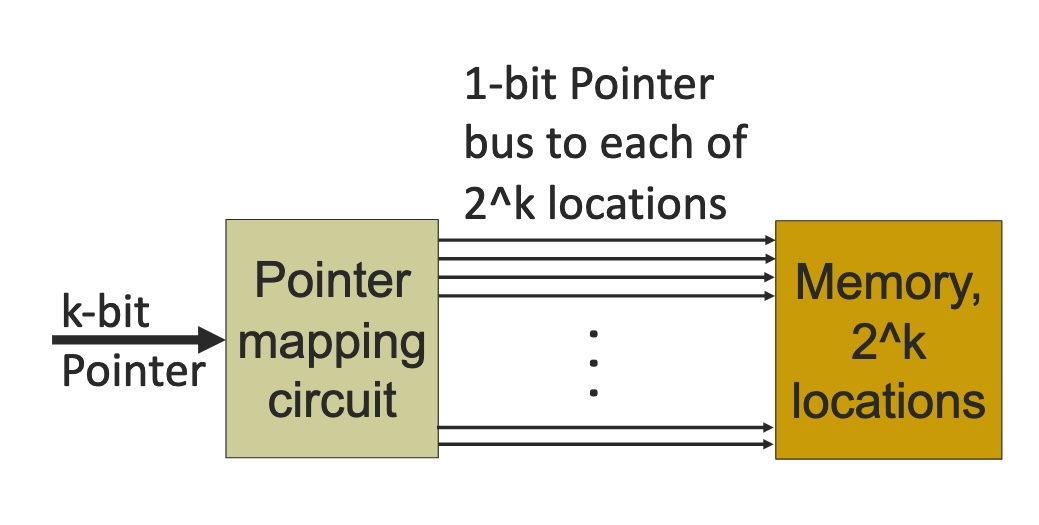
\includegraphics[width=.9\linewidth]{./img/pointing_function.jpg}
\caption{\label{fig:org0ec129b}Abstract Pointing Function Diagram}
\end{figure}

Memory chips are 2D, \(2^{k/2} \times 2^{k/2}\) grid creates \(2^k\) intersections -> Only \(2 * 2^{k/2}\) wires needed! Optimized design can reduce number of wires by \(\sqrt{2^k} / 2\)

\subsection{Register}
\label{sec:org235d5f8}

k-bit register has k latches to store \(2^k\) bit strings.

\section{Pointing}
\label{sec:org9374411}

\subsection{Decoder}
\label{sec:org2ce7f15}

A circuit with n wires input and 2\textsuperscript{n} wires output. Decoding output is selected or not\textsubscript{selected}

\begin{center}
\begin{tabular}{rrrrrr}
X & Y & D0 & D1 & D2 & D3\\
\hline
0 & 0 & 1 & 0 & 0 & 0\\
1 & 0 & 0 & 1 & 0 & 0\\
0 & 1 & 0 & 0 & 1 & 0\\
1 & 1 & 0 & 0 & 0 & 1\\
\end{tabular}
\end{center}

2-to-4 decoder truth table. \textbf{n inputs and 2\textsuperscript{n} outputs}.

\subsection{Selecting bus}
\label{sec:orga7b8fd4}

\begin{itemize}
\item \emph{Bus}: Group of n wires, carry n bit
\item \emph{Multiplexer (mux)}: Selects \textbf{from 2\textsuperscript{n} k-bit input buses, outputs to 1 k-bit output bus}
\item \emph{Demultiplexer (Demux)}: Reverse of mux
\end{itemize}
\end{document}